
In this section, I will provide logical explaination and statistical results,
illustrated as figures or tables, to address research questions mentioned in
\autoref{sec:research_questions}.

\subsection{RQ1: What types of stolen information are traded?}
%
As shown in \autoref{fig:type_allocation}, I captured in total 10 product types
based on my own standard. Among all categories, \emph{Personal Data} is the
most active field, contributing \(68,69\%\) of all traded items. \emph{Online Account}
represents the second larges portion \(17,73\%\). The rest of product types ranges
from \(0,36\%\) to \(3,45\%\). Detailed description of each product type is in
\autoref{tab:category_description}.

\begin{table}
    \centering
    \begin{tabularx}{\textwidth}{lX}
        \hline
        Product type & Description\\
        \hline
        Personal Data & Full name, date of birth, social security number, home
        address, zip code, driver license, employer info, etc.\\
        Online Account & Online account of services such as Netflix, Amazon,
        Venmo, Booking.com, etc.\\
        Bank Account & Username/password of online bank accounts, and credential
        information linked to bank accounts.\\
        Credit Card & Card holder name, \acrshort{cvv}, full name, address,
        bank name, card type.\\
        Passport & Real photos and scan of passports.\\
        Email & Emails leaked through data breaches.\\
        Lookup Service & \acrshort{ssn}/\acrshort{dob}/\acrshort{mmn}/\acrshort{dl}
        /\acrshort{cs} lookup service.\\
        Bank Identity Number & \acrshort{bin} is the first 6 digits of the credit card (with
        the help of this information you will understand what credit cards you need to
        work with 3-D Secure VBV) 3-D Secure VBV is a protocol that is used as an
        additional layer of security for online credit and debit cards, two-factor
        user authentication.\\
        Remote Desktop Protocol & The protocol provides user graphical interface to connect
        to other computers over the network connection~\cite{web:rdp_wiki}.\\
        Other & Tutorials, digital document templates, document forms, domains, etc.\\
        \hline
    \end{tabularx}
    \caption{Description of product types.}\label{tab:category_description}
\end{table}

\subsection{RQ2: What are the prices for different product types?}
%
There are 6/10 categories, providing more than 90\% of all traded items, 
recording the arithmetic mean price less than 20 USD\@. Furthermore, it supports
the numerical result of 15,87 USD (\autoref{tab:dataset_stat}), the average
price of the whole dataset. The average price of compromised emails is 158,5 USD,
the highest number over all product types. About 10\% of them are email leads,
being recorded 939,19 USD of average price. That explains why the average price
of email type is significantly higher than the overall mean price. In constrast,
products in \emph{Personal Data} field is observed the lowest average price ---
8,71 USD\@. It can be infered that regular Internet users are able to afford
others' indentity information at unexpected-low cost.

% \begin{figure}
%     \centering
%     \includegraphics[height=\textheight,width=\textwidth,keepaspectratio]
%     {plots/cate_prods_avg_price.png}
%     \caption{Number of products and average price over product types.}
%     \label{fig:cate_avg_prod}
% \end{figure}

\subsection{RQ3: Where the stolen information is from?}
%
The traded information is mainly from data breaches at high-traffic web
services. In \autoref{tab:data_breaches}, I collected a list of major data breaches.
A potential dataset from the breach is traded in Database marketplace, as shown
in \autoref{fig:best_buy_breach}. Information leaked through data breaches can be
email address, password, or more sensitive data, including banking account,
\acrshort{ssn}, and identity information. Moreover, exposed data can be utilized
in attacking campaigns that either trick victims to provide more their own personal
data or unauthorizedly access others account owned by the same user.

\begin{table}
    \begin{tabularx}{\textwidth}{| X | X | X |}
        \hline
        Name of service & Year & Number of victims\\
        \hline
        Capital One & 2019 & 100 million Americans and 6 million Canadians\\
        Yahoo & 2013, 2014 & 3 billion, 500 million\\
        Marriott International & 2018 & 500 million\\
        First American Financial & 2019 & 885 million\\
        Facebook & 2019 & 540 million\\
        % \[[24]\]7.ai --- Bestbuy, Sears, Delta & 2017 & Sears: 100000, Delta: several hundred
        % thoudsands, Bestbuy: ``a small fraction of online customers''
        \hline
    \end{tabularx}
    \caption{List of major data breaches~\cite{web:best_buy_breach,web:capital_one_breach,
    web:personal_info_darkweb}.}\label{tab:data_breaches}
\end{table}

\begin{figure}
    \centering
    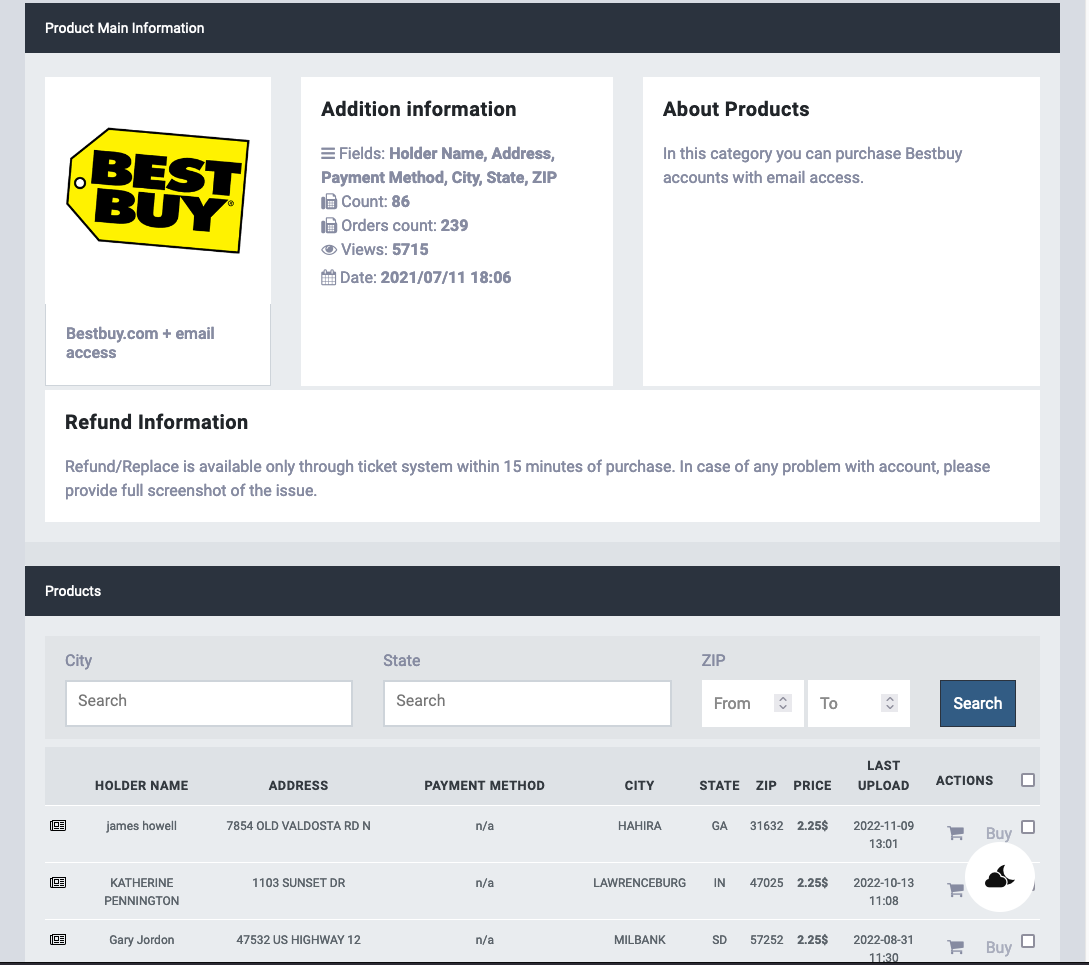
\includegraphics[width=\textwidth,height=\textheight,keepaspectratio]
    {screenshots/best_buy_info.png}
    \caption{Leaked information of Bestbuy's customer.}\label{fig:best_buy_breach}
\end{figure}

\subsection{RQ4: What we can learn about the sellers?}
%
In general, there are two types of sellers, a store sells a large amount of low-cost
items and the one provides a small amount of expensive products (\autoref{fig:avg_prods_seller}).
In anonymous marketplaces, personal contacts of the vendors are unavailable.
To become a seller, a visitor has to provide a list of his/her available products.
Moreover, feedbacks from other anonymous forums and markeplaces need to be sent
to administrators of Database market to prove that the applicant is a valid merchant.

\begin{figure}
    \centering
    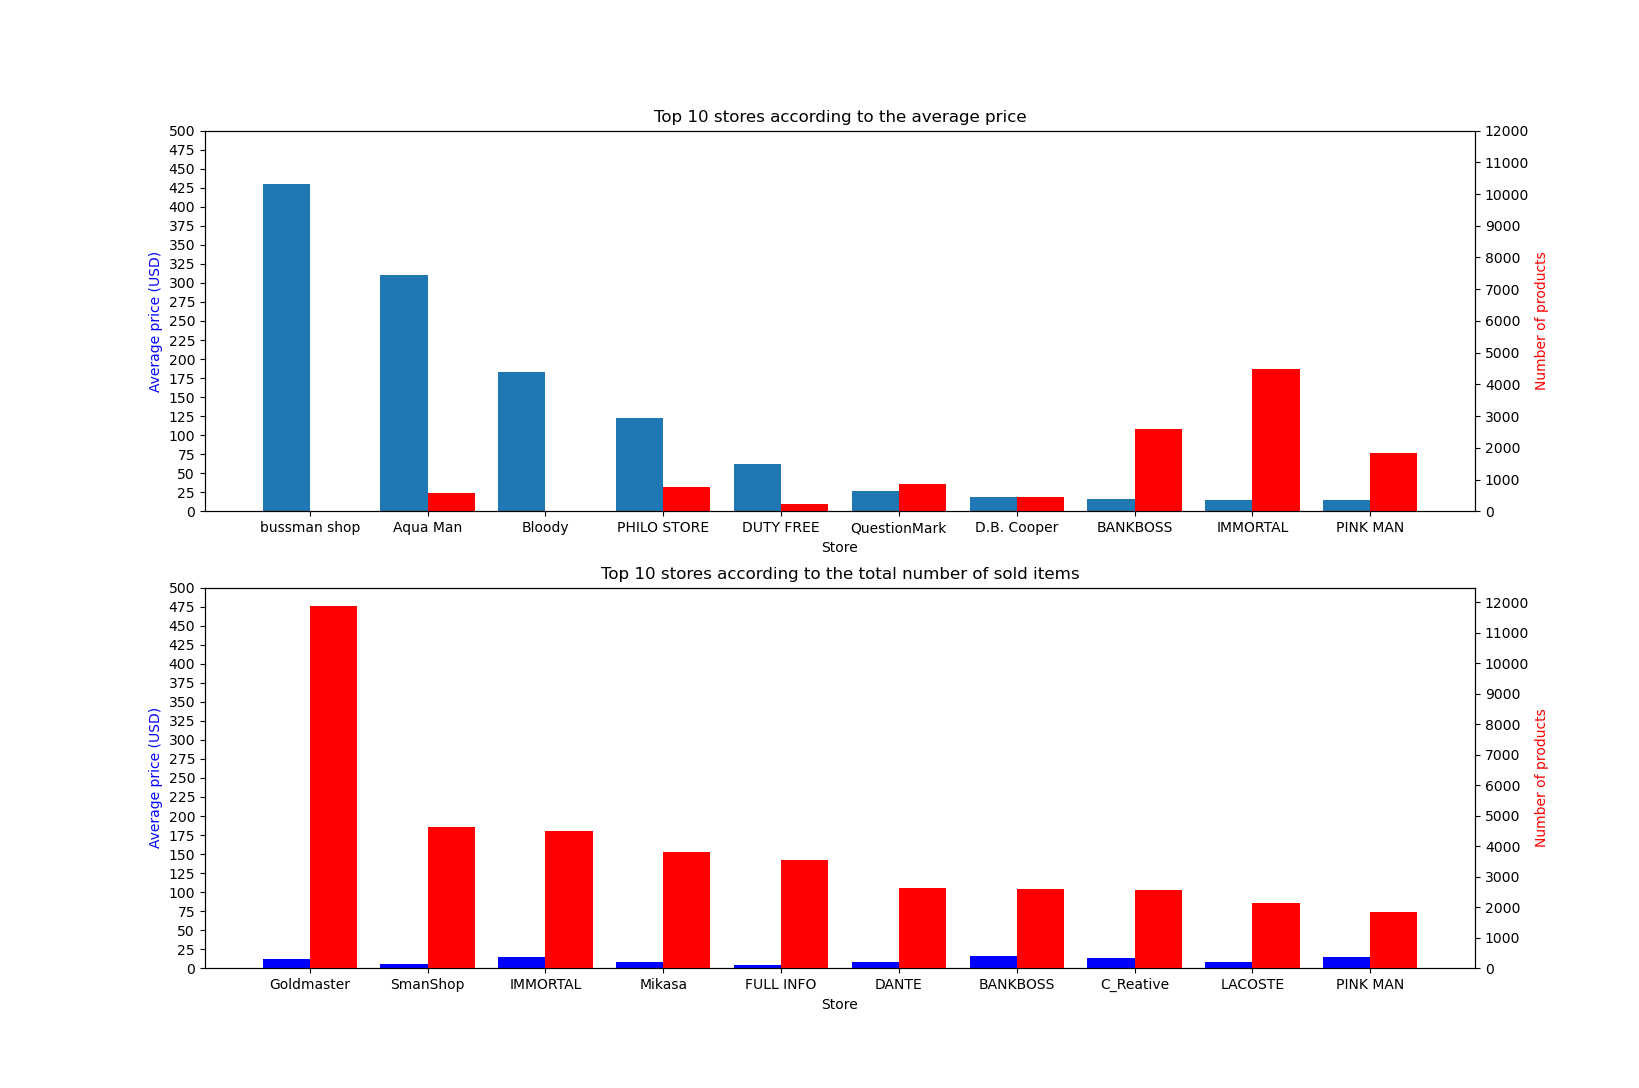
\includegraphics[width=\textwidth,height=\textheight,keepaspectratio]
    {plots/top_avg_price_num_prods_seller.png}
    \caption{Top sellers sorted based on the average price and total number
    of traded products.}\label{fig:avg_prods_seller}
\end{figure}